\documentclass[]{article}

\usepackage{graphicx}
\usepackage[margin=3cm]{geometry}

\graphicspath{{images/}}

%opening
\title{koda: Deep Learning-Enhanced Pipeline for Keyword Detection in Document Images} 
\author{Matteo Pellegrino, Federico Terzi}

\begin{document}

\maketitle

\begin{abstract}
TODO
\end{abstract}

\section{Introduction}
TODO


\section{Edge Detection}

Above all the possible approaches, the pipeline proposed in this paper heavily
relies on edges to detect documents inside images. Therefore, in order to obtain
good results, it is crucial to employ a solid \textit{edge detection} algorithm.


\subsection{First Attempts with Canny}

Our initial attempts to detect document edges involved the well known \textit{Canny edge detector} [TODO REF]. Although applying the filter directly does detect the sheet edges, it presents many artifacts
due to the text printed on the document itself (as seen in Fig. \ref{fig:canny_gaussian} (B)).

In order to mitigate the problem, a \textit{Gaussian filter} [TODO REF] is applied before the edge detection, obtaining a clear highlighting of the interesting edges (as seen in Fig.  \ref{fig:canny_gaussian} (C)).

\begin{figure*}[!htb]
	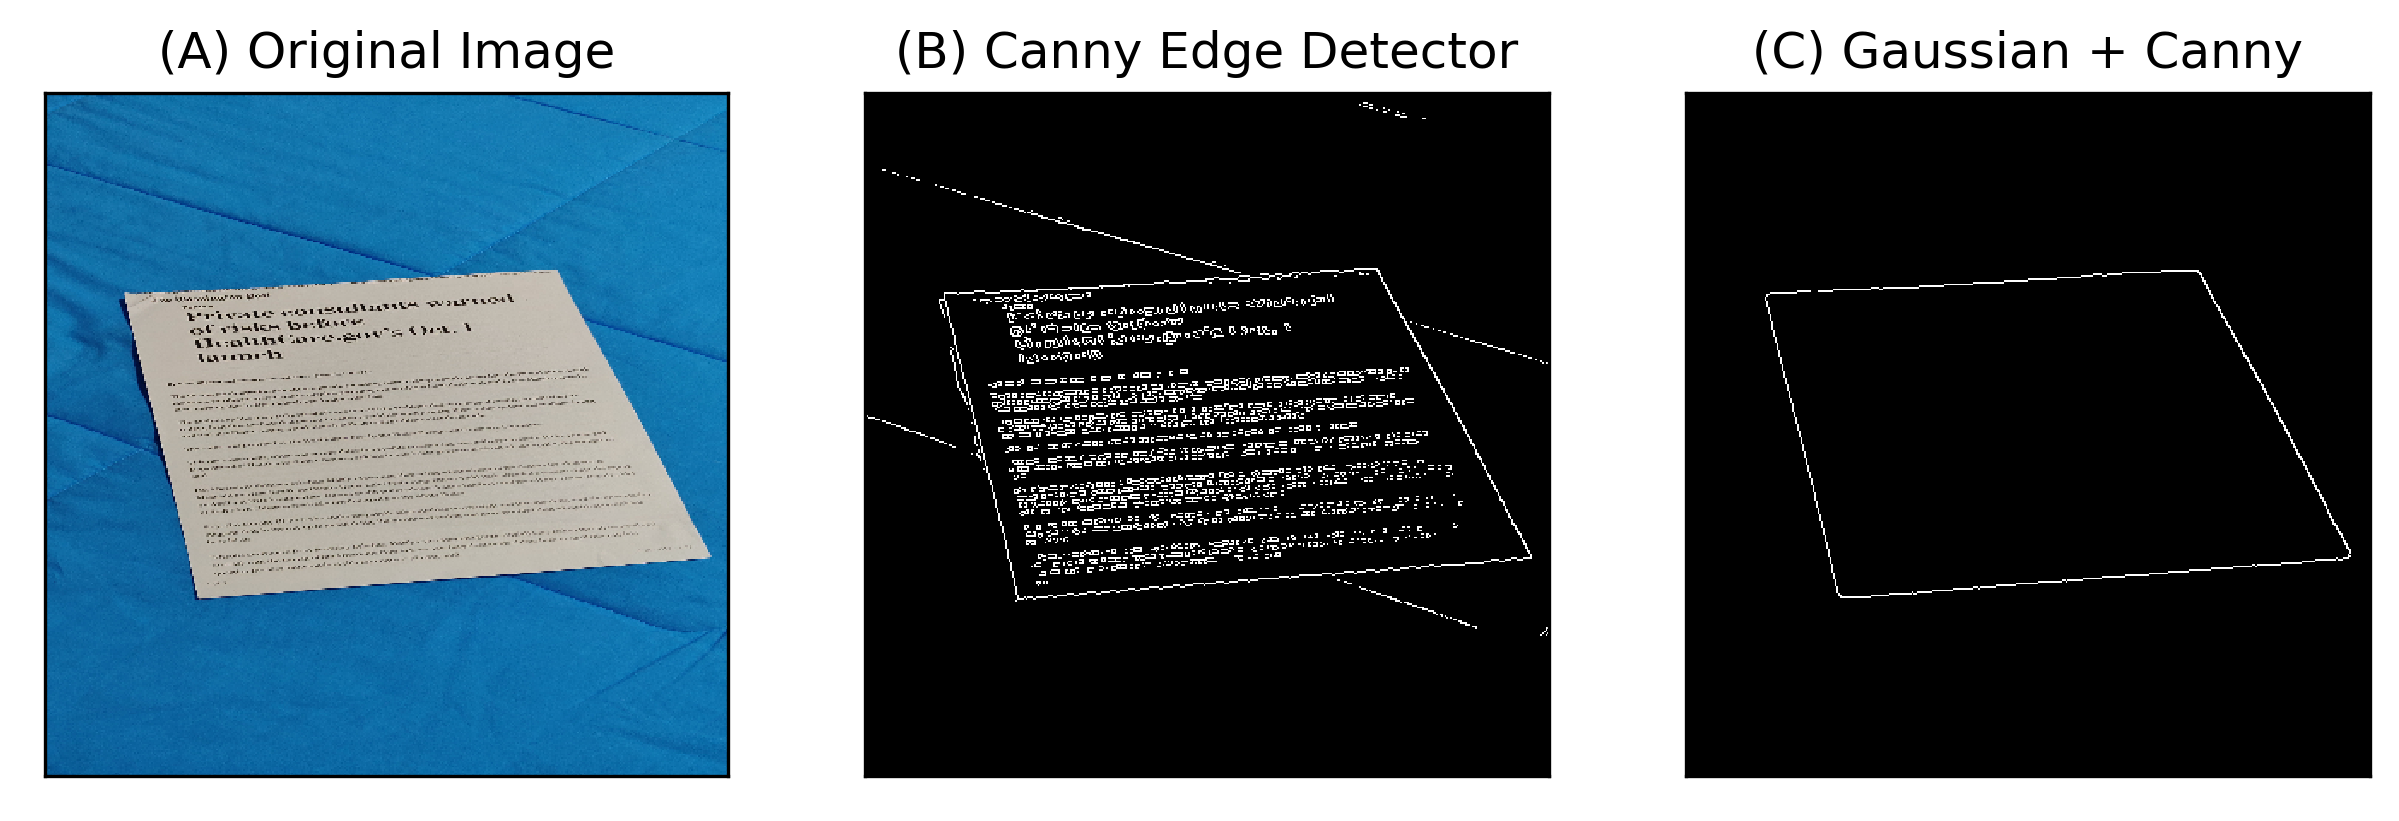
\includegraphics[width=\linewidth]{canny_gaussian.png}
	\caption{TODO}
	\label{fig:canny_gaussian}
\end{figure*}

Despite the result, after many observations it became clear that this approach was not robust enough to
work in all real-world scenarios. In particular, Canny's parameter tuning turned out to be a major
problem, as it can be seen in Fig \ref{fig:canny_comparison}, where a combination of parameters,
despite producing good results in some scenarios, proved itself incapable of generalizing well in others.

\begin{figure*}[htb!]
	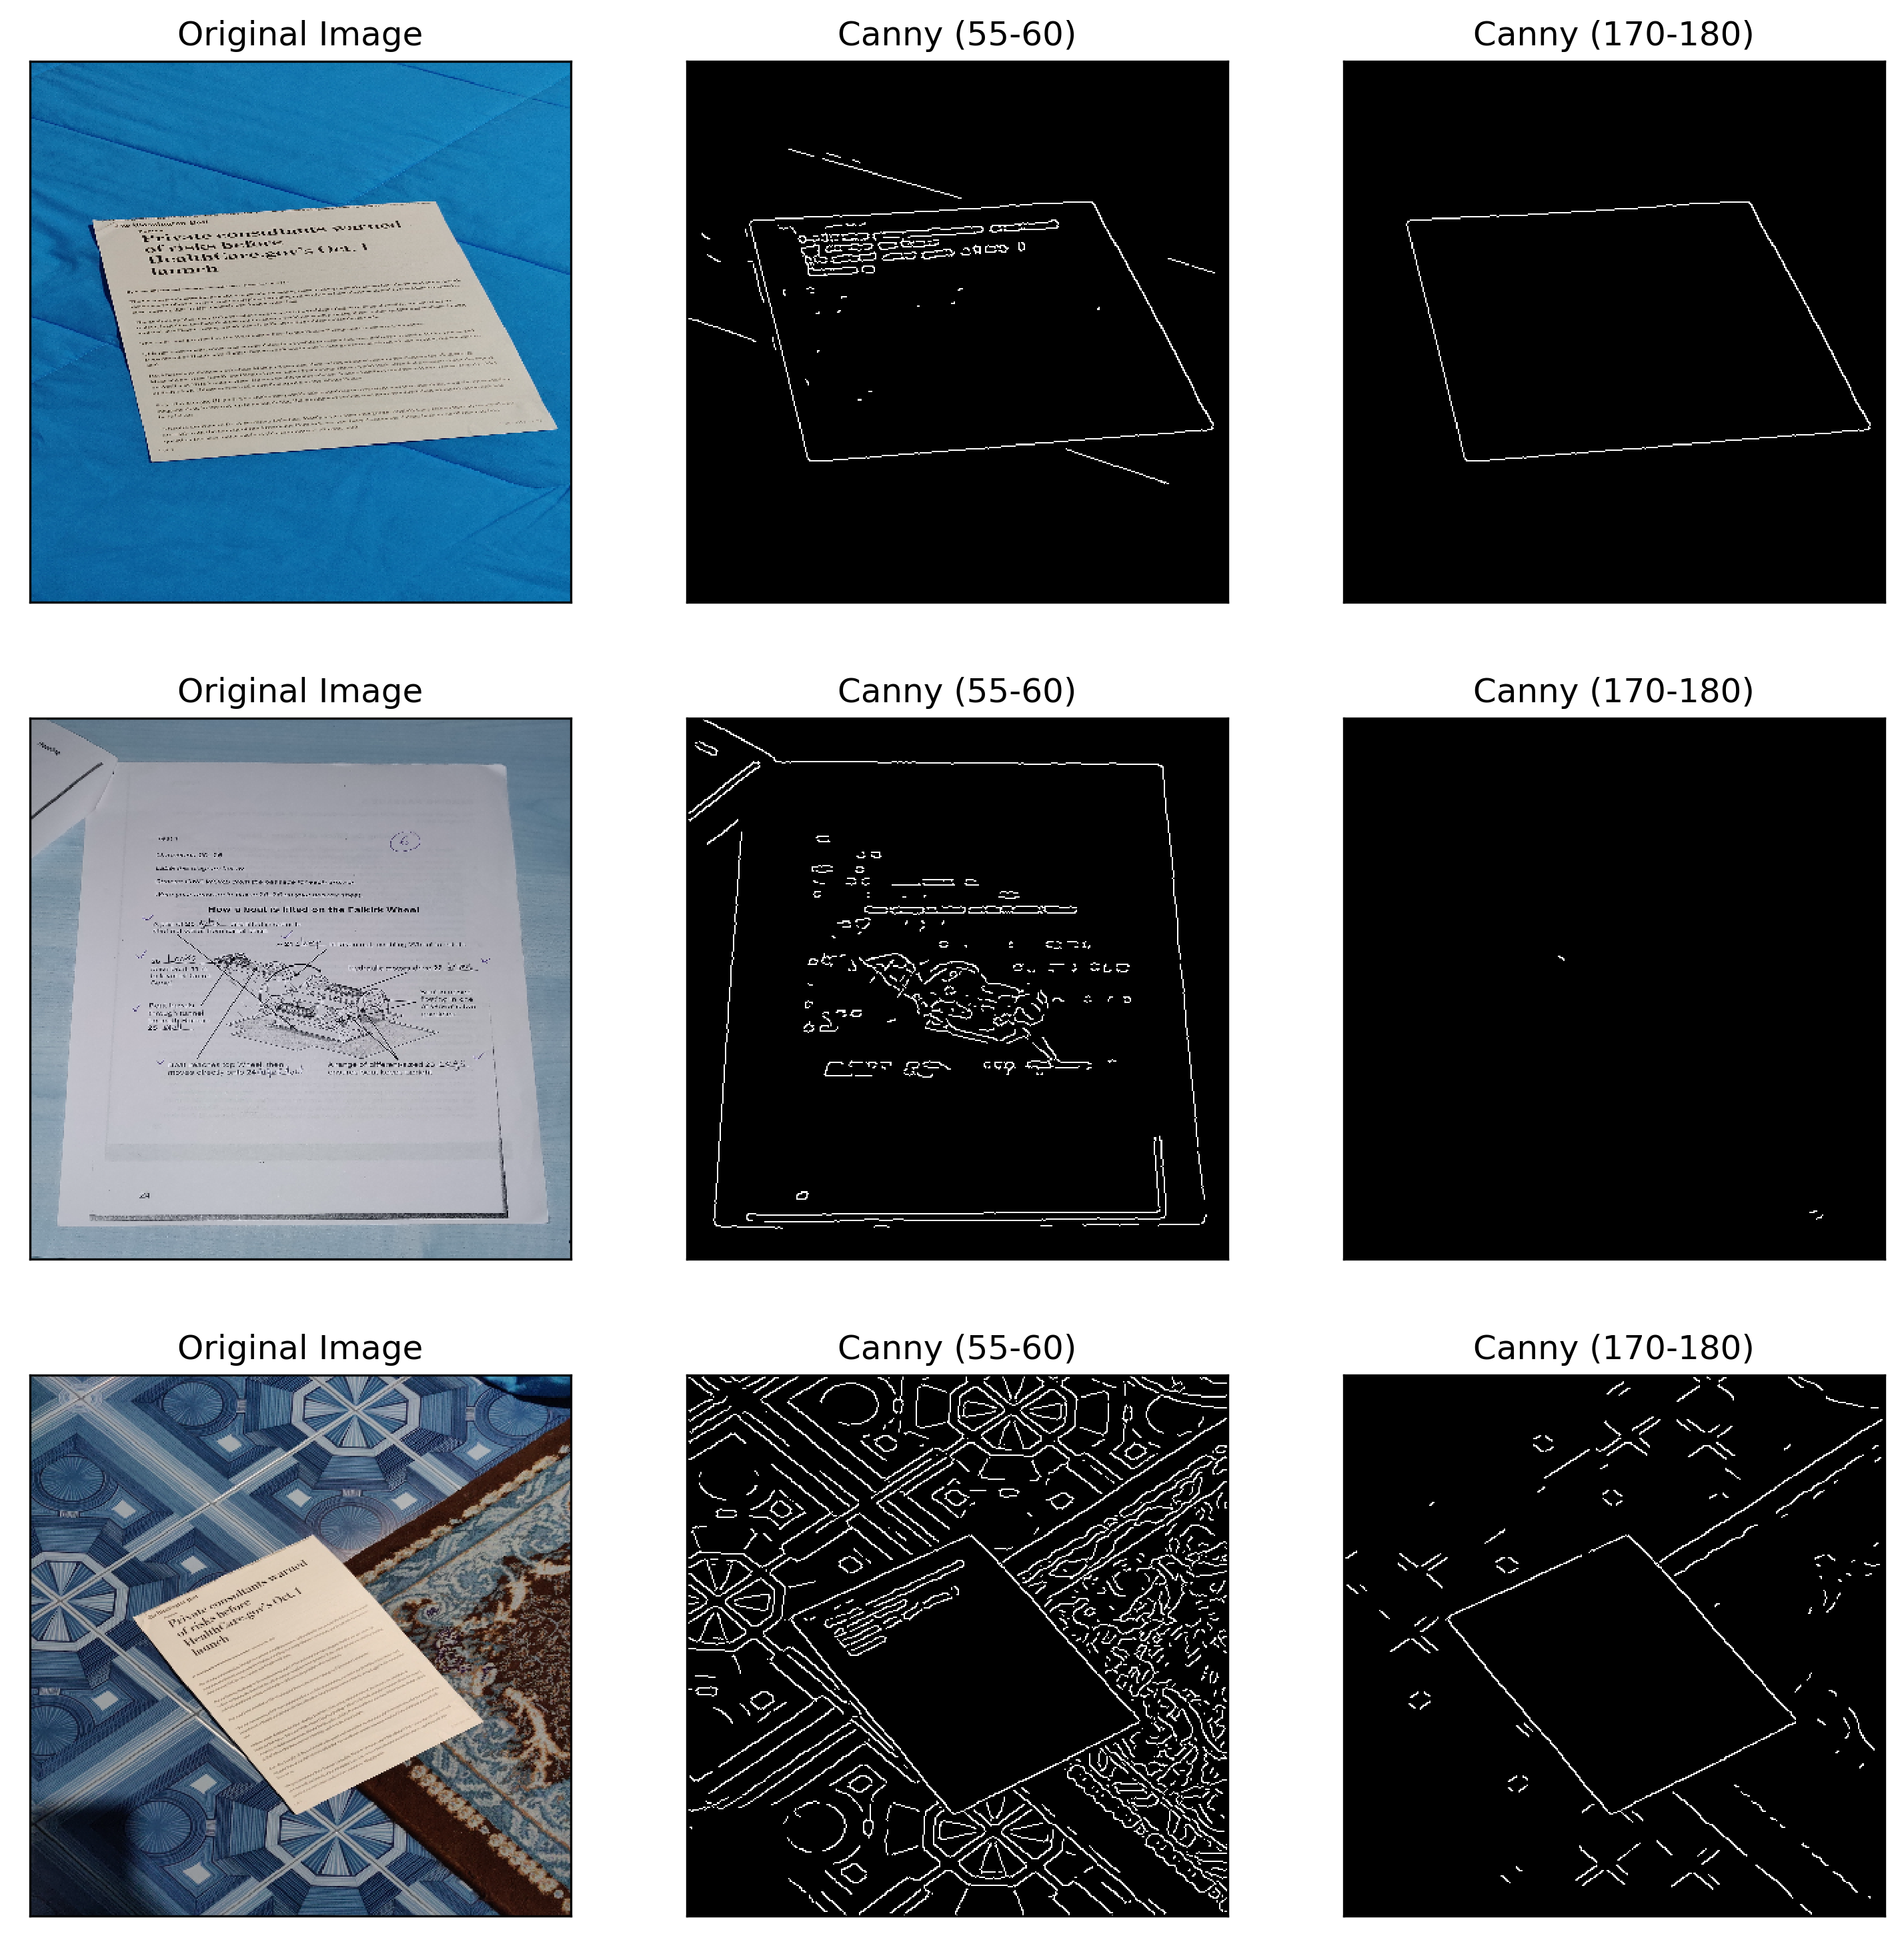
\includegraphics[width=\linewidth]{canny_comparison.png}
	\caption{TODO}
	\label{fig:canny_comparison}
\end{figure*}

\subsection{Deep Learning Approach}

In order to make the pipeline able to deal with real-world images, it is crucial to develop an
edge detection mechanism capable of generalizing better in heterogeneous situations. 
For this reason, a \textit{Deep Learning}-based approach was explored with the aim of creating a model
capable of distinguishing document sheet edges from the rest of the image.

Due to the lack of a suitable dataset with labelled document edges, a custom one was created.
In particular, 250 images containing document sheets were taken under different lighting conditions, 
backgrounds and positions. Thereafter, every image was labelled with the 4 corner coordinates of the document.

For this particular task, \textit{Keras}, an open-source Python library for Deep Learning [TODO REF], was chosen to build the model. Many experiments were made to find the right architecture, most of them 
exploiting \textit{convolutional neural networks}. Above all of them, KODA uses \textit{U-Net}[TODO REF], a popular architecture for \textit{object segmentation}, and in particular an open-source implementation for Keras [TODO REF].

The model takes a 3-dimensional input image (RGB) and outputs a 2-d map of the edges. Although the shape
of those matrices can vary, KODA uses a 256 pixels side for both input and output, as it provides a reasonable compromise between size and resolution. Fig. \ref{fig:label_edge} illustrates the way a
sample is fed to the network. In particular, the input image is resized to a 256x256 RGB image and the
output label is a gray scale map of the expected document edges.

\begin{figure*}[htb!]
	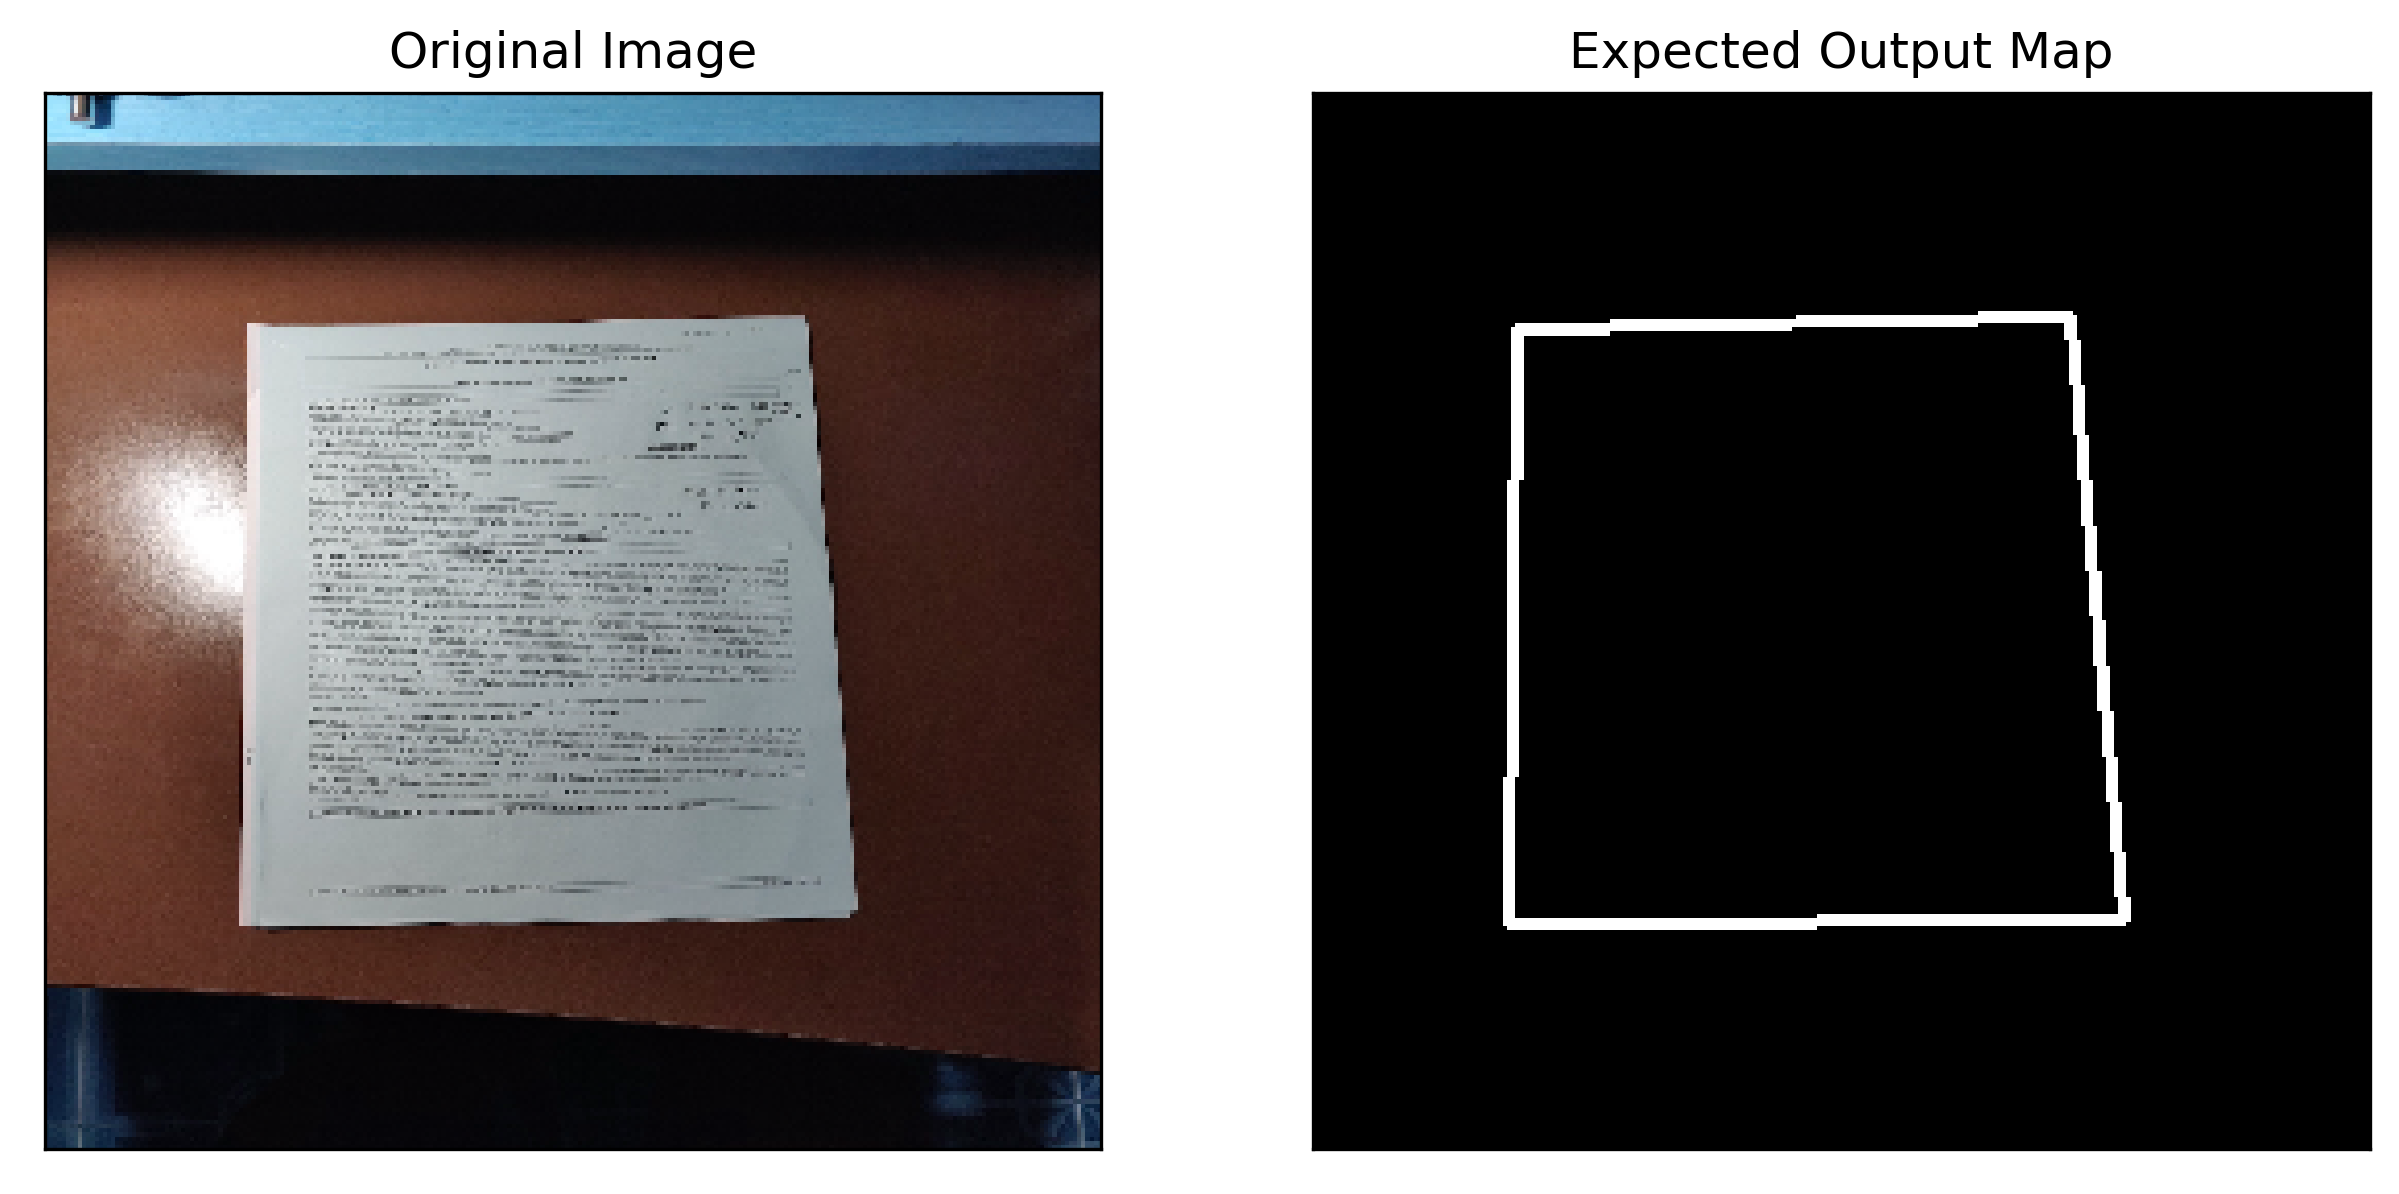
\includegraphics[width=\linewidth]{label_edge.png}
	\caption{Example of the way a sample is fed to the network.}
	\label{fig:label_edge}
\end{figure*}

Due to the high number of required samples, the dataset itself is insufficient to fully train the network.
For this reason, a technique called \textit{data augmentation}[TODO REF] is applied to provide the model
with enough variability. In particular, before being fed to the network, a random combination of transformations, such as scale, translation, rotation and brightness changes, is applied to the image and to the resulting edge feature map, as shown in Fig. \ref{fig:augmented_image}.

\begin{figure*}[htb!]
	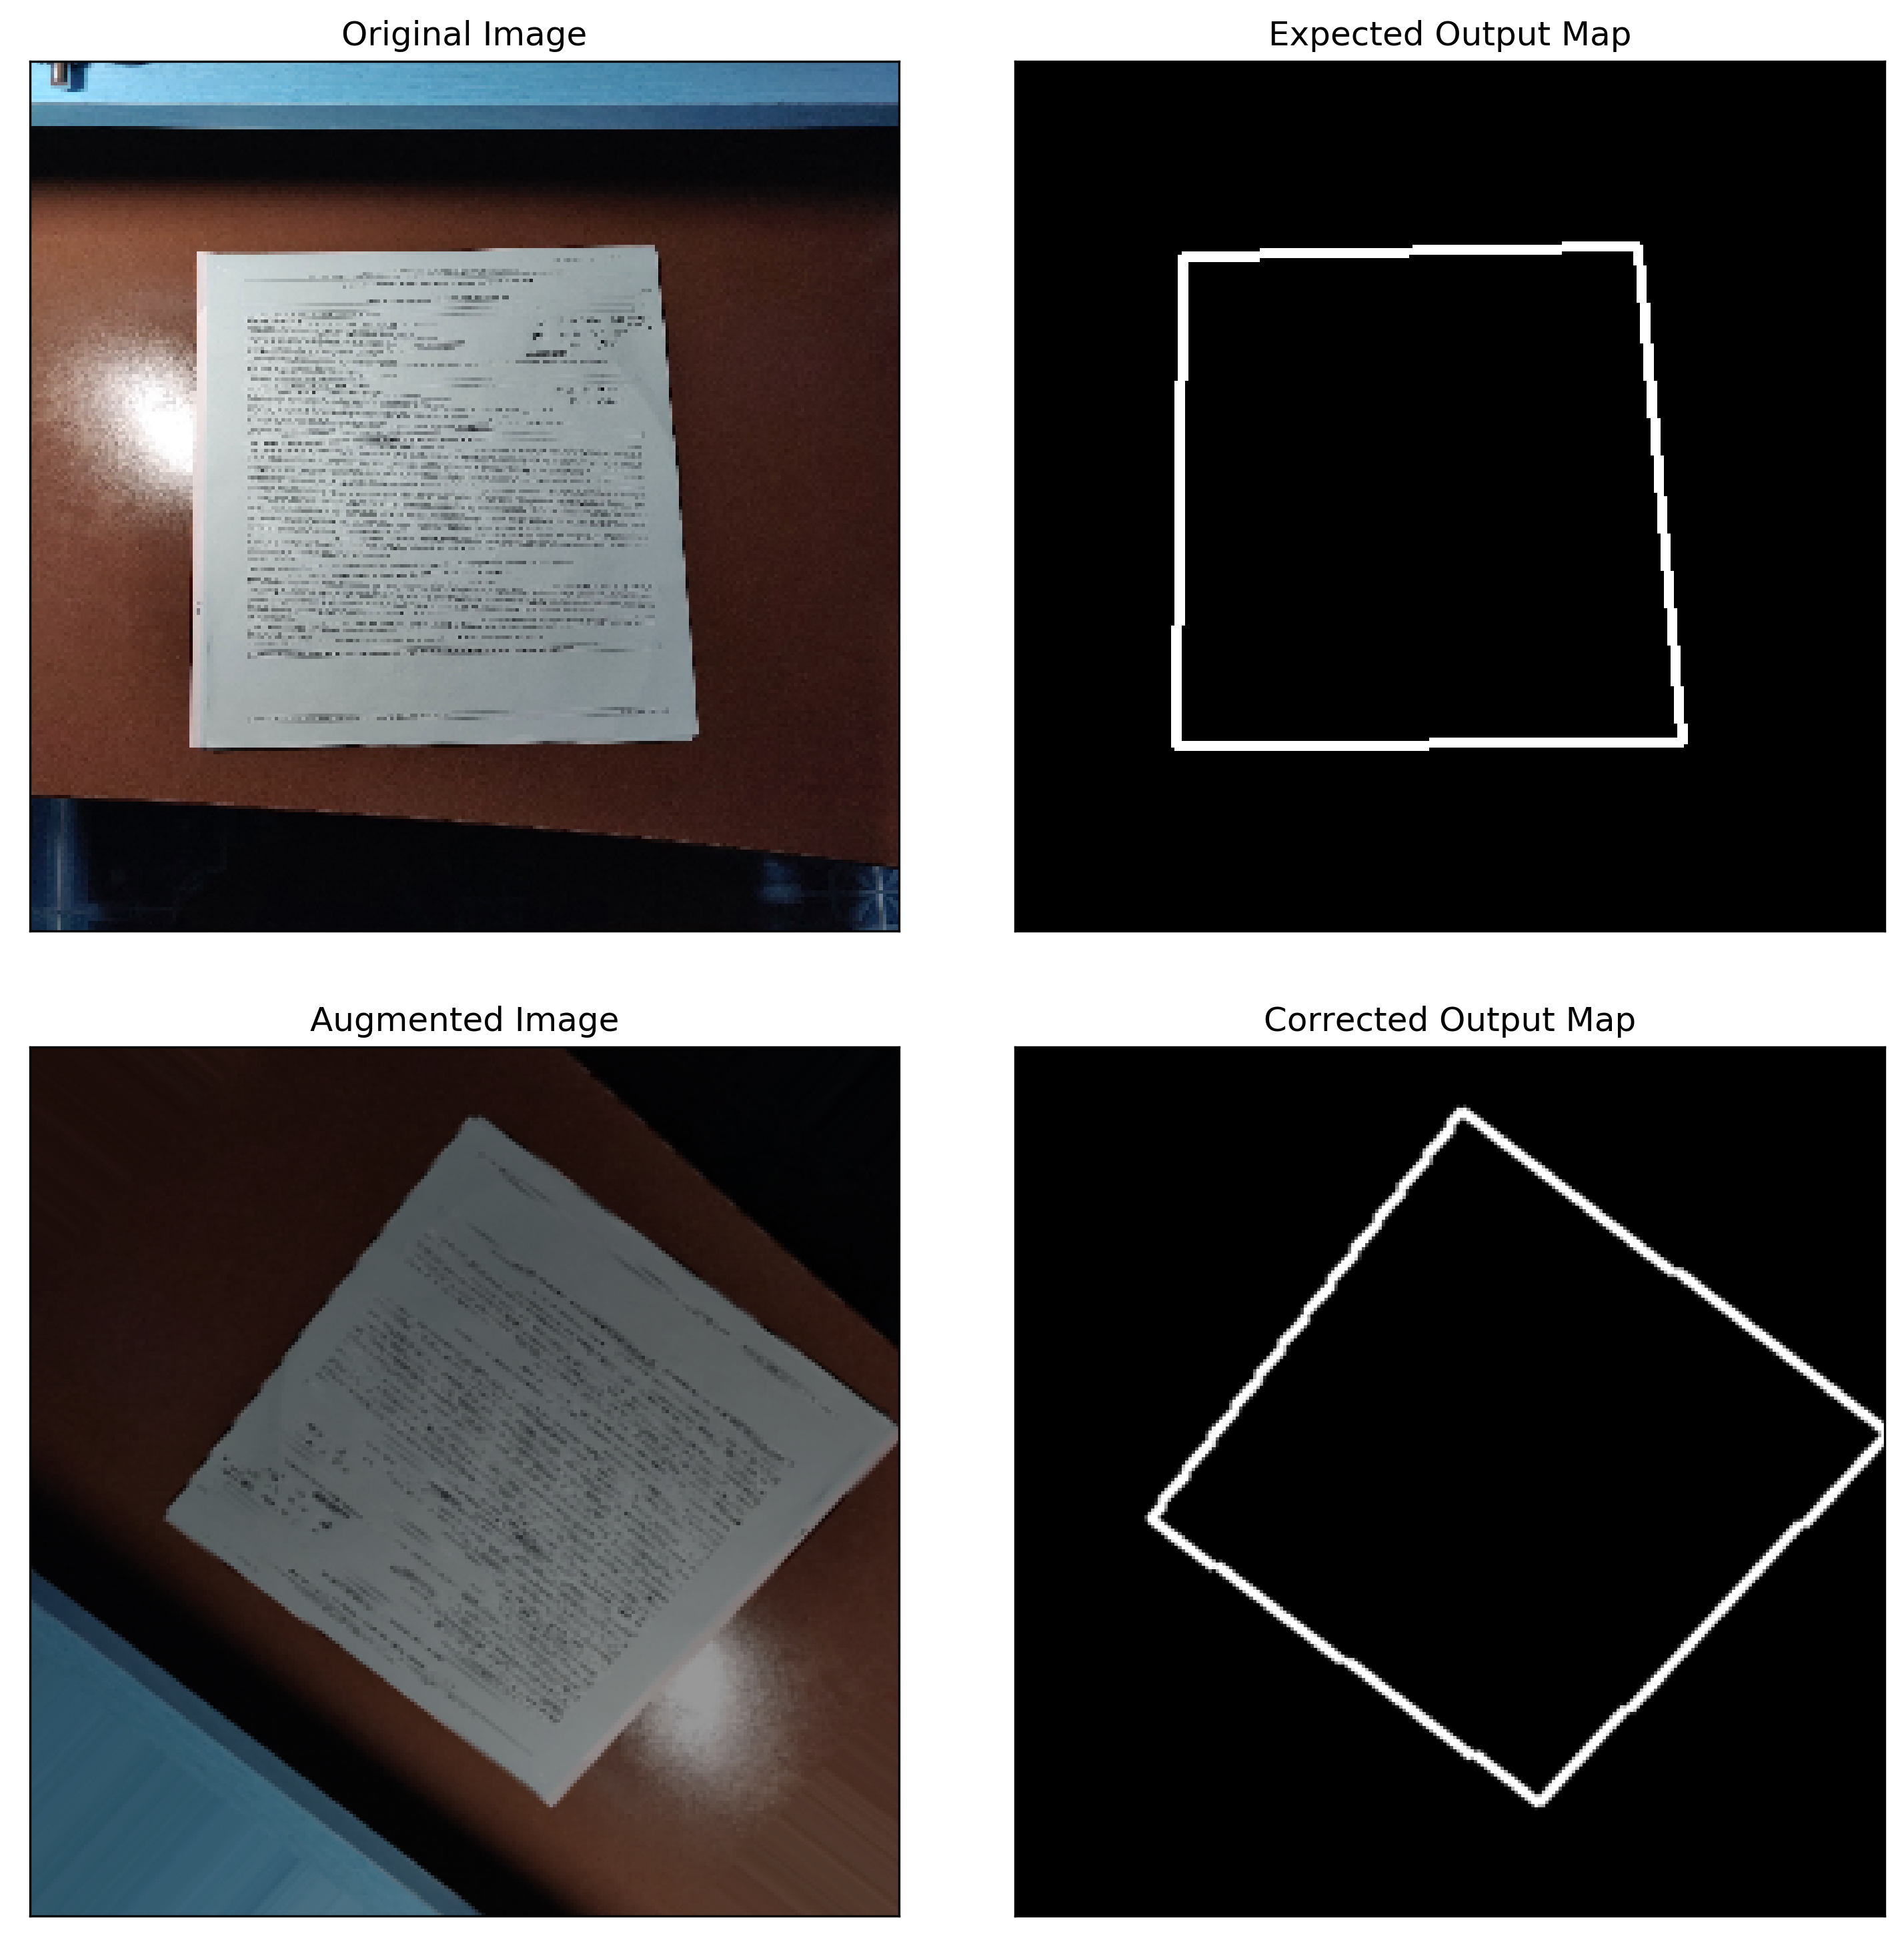
\includegraphics[width=\linewidth]{augmented_image.png}
	\caption{Example of Data Augmentation}
	\label{fig:augmented_image}
\end{figure*}



\end{document}
